\section{Hamiltonian comparison}\label{sec:cmp}

This section produces a comparison datum (Definition~\ref{def:mech-datum}) for the profile of $k\ge10$ equal balls.
Let $h>0$, $\bar D(h)=\{w\in\C:p(w)\le h\}$ with $p=\pi|w|^2$, $\theta=\arg w/2\pi$ and $\omega_V=dp\wedge d\theta$
(\S\ref{sec:mech}), and let $P$ be continuous and concave on $[0,h]$ with positive mean. We seek a smooth $K$ and a
Hamiltonian isotopy $q_t$ of $\bar D(h)$ with $(K-P)\circ p\circ q_1\le K\circ p-\gamma$ for some $\gamma>0$. Since
$p_*\omega_V$ is Lebesgue measure on $[0,h]$, $q_1$ only redistributes the values of $K-P$.

The rearrangement operator is that of \cite[\S2]{OpenAI2026}, where $K$ is the fixed point of a contraction built
from it. For $k\ge10$ equal balls, \S\ref{sec:cmp-linear} gives a closed-form datum with linear $K$ and no fixed
point. Everything is explicit at level L1 (Definition~\ref{def:intro-levels}).

\subsection{The increasing rearrangement}\label{sec:cmp-rearrangement}

\begin{definition}[Increasing rearrangement]\label{def:cmp-rearrangement}
For a continuous convex function $F$ on $[0,h]$ put
\[
 (R_1F)(x)=\min_{0\le a\le h-x}\ \max\bigl(F(a),\,F(a+x)\bigr),\qquad 0\le x\le h .
\]
\end{definition}

The minimum exists, and since sublevel sets of convex functions are intervals, $R_1F$ is the increasing rearrangement
of $F$ on $[0,h]$. The properties used below are in
\Sref{Lemma}{lem:fcp-rearrangement}: $R_1$ is monotone, commutes with adding constants and with multiplication by
$\alpha\ge0$, and preserves integrals and maxima.

\subsection{The linear comparison identity}\label{sec:cmp-linear}

For $k\ge10$ equal capacities in dimension four no fixed point is needed. The height $h=t_0/3$ is chosen so that,
for linear $K$, the function $K-P$ is a constant plus a multiple of a tent that takes the same value at both ends of
$[0,h]$. Each sublevel interval of such a tent has length equal to its level, so its increasing rearrangement is the
identity, and the comparison inequality reduces to a constant gap. This datum serves \Sref{Theorem}{thm:cub-packing}.

Here $\Delta=[0,h]$ with $h$ real (rationality is not used), so $V_\Delta=\bar D(h)$. The symbols $s,a,c_s,g,A,B$ are local to this subsection and to \Ssec{sec:fcp-equal}. For an integer $k\ge10$ and $\eta_\star\in(0,\frac14)$, set $t_0=1-\eta_\star/2$ and
\[
s=\sqrt k,\quad a=\frac{t_0}s,\quad h=\frac{t_0}3,\quad c_s=3s-9,\quad g=3(1-t_0),\quad A=\frac ha,\quad B=\frac h{h-a}.
\]
Since $s>3$, we have $0<a<h$, $c_s>0$, $A,B>0$, and
\begin{equation}\label{eq:cmp-AB}
\frac1A+\frac1B=\frac ah+\frac{h-a}h=1 .
\end{equation}
Let $\Lambda(x)=A(a-x)$ for $x\le a$ and $\Lambda(x)=B(x-a)$ for $x\ge a$. This is a tent with $\Lambda(0)=\Lambda(h)=h$ and $\Lambda(a)=0$.

\begin{lemma}[Sublevel sets of the tent]\label{lem:cmp-tent-sublevel}
\lean{SymplecticPacking.Params.Rcal_le_iff, SymplecticPacking.Params.sublevel_length,
SymplecticPacking.Params.sublevel_subset, SymplecticPacking.Params.volume_sublevel}
\uses{eq:cmp-AB}
For $b\ge0$, $\{x\in\R:\Lambda(x)\le b\}=[a-b/A,\,a+b/B]$, an interval of length $b$. If $b\le h$, it is
contained in $[0,h]$.
\end{lemma}

\begin{proof}
The interval is read off from the two affine pieces. Its length is $b(1/A+1/B)=b$ by \eqref{eq:cmp-AB}. If $b\le h$, then $a-b/A\ge a-h/A=0$ and $a+b/B\le a+h/B=h$.
\end{proof}

\begin{corollary}[Rearrangement of the tent]\label{thm:cmp-tent-rearrangement}
\uses{lem:cmp-tent-sublevel, def:cmp-rearrangement}
On $[0,h]$, $R_1\Lambda(x)=x$ for $0\le x\le h$. Consequently
$R_1(-g+c_s\Lambda)(x)=-g+c_sx$.
\end{corollary}

\begin{proof}
With $\alpha=a-x/A$ we have $\alpha\ge0$, $\alpha+x=a+x/B\le h$ and $\Lambda(\alpha)=\Lambda(\alpha+x)=x$, so $R_1\Lambda(x)\le x$. Conversely, suppose an admissible $[\alpha,\alpha+x]$ had $b'=\max(\Lambda(\alpha),\Lambda(\alpha+x))<x$. By convexity it would lie in $\{\Lambda\le b'\}$, which has length $b'<x$ (Lemma~\ref{lem:cmp-tent-sublevel}); this is impossible. The second claim follows from Lemma~\Snum{lem:fcp-rearrangement}(iv), since $c_s>0$.
\end{proof}

\begin{figure}[ht]
\centering
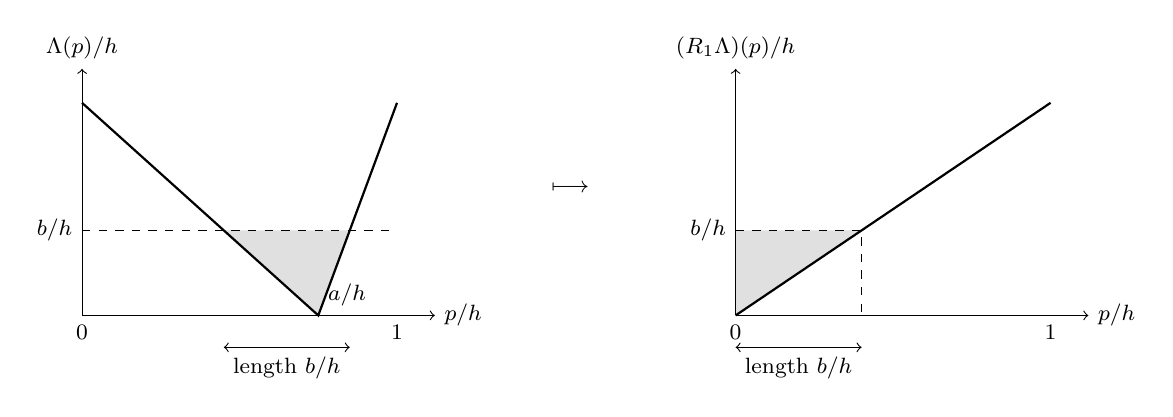
\begin{tikzpicture}[x=4cm,y=2.7cm,font=\footnotesize]
 \begin{scope}
 \fill[black!12] (0.45,0.4) -- (0.75,0) -- (0.85,0.4) -- cycle;
  \draw[->] (0,0) -- (1.12,0) node[right] {$p/h$};
  \draw[->] (0,0) -- (0,1.16) node[above] {$\Lambda(p)/h$};
  \draw[thick] (0,1) -- (0.75,0) -- (1,1);
  \draw[dashed] (0,0.4) node[left] {$b/h$} -- (1,0.4);
  \draw[<->] (0.45,-0.15) -- (0.85,-0.15) node[midway,below] {length $b/h$};
  \node[below] at (0,0) {$0$};
  \node[below] at (1,0) {$1$};
  \node[above right] at (0.75,0) {$a/h$};
 \end{scope}
 \node at (1.55,0.6) {$\longmapsto$};
 \begin{scope}[xshift=8.3cm]
  \fill[black!12] (0,0) -- (0,0.4) -- (0.4,0.4) -- cycle;
  \draw[->] (0,0) -- (1.12,0) node[right] {$p/h$};
  \draw[->] (0,0) -- (0,1.16) node[above] {$(R_1\Lambda)(p)/h$};
  \draw[thick] (0,0) -- (1,1);
  \draw[dashed] (0,0.4) node[left] {$b/h$} -- (0.4,0.4) -- (0.4,0);
  \draw[<->] (0,-0.15) -- (0.4,-0.15) node[midway,below] {length $b/h$};
  \node[below] at (0,0) {$0$};
  \node[below] at (1,0) {$1$};
 \end{scope}
\end{tikzpicture}
\caption{The linear comparison: the sublevel interval of $\Lambda$ has length $b$, so its increasing rearrangement
is $p$. The drawing uses $a/h=3/4$ ($k=16$); the identity holds for every $k\ge10$.
Consequently $K-R_1(K-P)\equiv g$, before the planar realisation error is deducted.}
\label{fig:cmp-tent}
\end{figure}

\begin{proposition}[Linear comparison datum for equal balls]\label{prop:cmp-linear}
\lean{SymplecticPacking.Params.F_eq, SymplecticPacking.Params.margin_one,
SymplecticPacking.Params.K_sub_F_ge, SymplecticPacking.Qhat.K_sub_F_q_ge,
SymplecticPacking.Qhat.full_comparison, SymplecticPacking.Qhat.qhatP_spec,
SymplecticPacking.Branch2.CubicData.ofParams_valid}
\uses{lem:cmp-tent-sublevel, thm:cmp-tent-rearrangement, def:mech-datum, S-lem:fcp-AB, S-def:fcp-eq, S-thm:pll-inner}
With the notation above let $\Delta=[0,h]$, $P(p)=3(1-3p)-k(a-p)_+$, $K(p)=c_sp$ and $F=K-P$. Then
\begin{equation}\label{eq:cmp-identity}
 F(x)=-g+c_s\Lambda(x)\qquad(x\in\R).
\end{equation}
Let $e_q=\min\bigl(h/100,\ g/(128c_s)\bigr)$ (\Sref{Definition}{def:fcp-eq}) and let $(q_t)$ be the isotopy of
\Sref{Theorem}{thm:pll-inner}, whose endpoint $q=q_1$ satisfies $\Lambda(p(q(z)))\le\pi|z|^2+4e_q$ on $\bar D(h)$.
Then $(K,(q_t))$ is a comparison datum for $(\Delta,P)$ with gap $\tfrac{31}{32}g$.
\end{proposition}

\begin{proof}
By \Sref{Lemma}{lem:fcp-AB}, $c_sA=k-3s$, $c_sB=3s$ and $3sa=3-g$. Hence both sides of \eqref{eq:cmp-identity} equal $(3s-k)x+ka-3$ for $x\le a$, and $3sx-3$ for $x\ge a$.

By \Sref{Theorem}{thm:pll-inner}, $q_0=\mathrm{id}$ and each $q_t$ maps $\bar D(h)$ onto itself. Moreover $q_t=\mathrm{id}$ and $Q_t=0$ on $\{\pi|z|^2>P_{\rm supp}\}$ for a constant $P_{\rm supp}<h$; this gives condition~\ref{it:mech-datum-collar} of Definition~\ref{def:mech-datum}.

For condition~\ref{it:mech-datum-cmp}, let $w\in\bar D(h)$ and $I=p(w)$. By \eqref{eq:cmp-identity} and $4c_se_q\le g/32$,
\[
K(I)-(K-P)\bigl(p(q(w))\bigr)=c_sI+g-c_s\Lambda\bigl(p(q(w))\bigr)\ge g-4c_se_q\ge\tfrac{31}{32}g .\qedhere
\]
\end{proof}

Thus $K-R_1F\equiv g$ exactly (Corollary~\ref{thm:cmp-tent-rearrangement}), and the planar map costs at most $g/32$. Ideally $q$ would carry each centred disc $\bar D(b)$, $0\le b\le h$, onto the sublevel set
$\{\Lambda\circ p\le b\}=\{a-b/A\le p\le a+b/B\}$, an annulus (a disc for $b=h$) of the same area $b$, nested in $b$; no
area-preserving homeomorphism does this exactly (\Ssec{sec:fcp-equal}). The map of \Sref{Theorem}{thm:pll-inner} is
built from Morse charts of a smoothed tent potential. On the core $\bar D(h-\frac{31}8e_q)$ its error is below
$\frac{13}{24}e_q$; the full loss $4e_q$ occurs only on the outer annulus, where $q$ is joined to the identity.
In \cite{OpenAI2026} the comparison function is the fixed point of the contraction $T_\lambda$ and the gap comes from
the contraction argument; here the identity~\eqref{eq:cmp-identity} gives it directly. As $t_0\to1$, $g\to0$ while
$ka^2=t_0^2\to1$. The equal-capacity branch takes $\eta_\star=1-\rho\sqrt k$, so $t_0=(1+\rho\sqrt k)/2$ and
$g=3\eta_\star/2$.

\begin{remark}[The range of the linear datum]\label{rem:cmp-small-k}
The linear comparison is used when the capacities are equal, $k\ge10$ and $\eta_\star=1-\rho\sqrt k$ lies in
$(0,\frac14)$, that is $\frac34<\rho\sqrt k<1$. For $k=9$ the formulas give $a=h$, and for unequal capacities a
linear $K$ can fail; these inputs use the scalar comparison datum of the companion paper~\cite{SongHD}.
\end{remark}
